\documentclass[]{report}
\usepackage[backend=bibtex,style=ieee]{biblatex}
\usepackage{xcolor}
\usepackage{graphicx}
\usepackage{csquotes}
\usepackage{url}
\usepackage{amsmath}
\usepackage[]{hyperref}
\usepackage{xurl}
\usepackage{booktabs}
\usepackage{listings}
\lstset{numbers=none,basicstyle=\footnotesize\ttfamily,breaklines=true}
\usepackage{url}
\usepackage{varwidth}
\usepackage[hang]{footmisc}

\begin{filecontents}{ref.bib}
    @misc{izhikevich2023democratizing,
    title         = {Democratizing LEO Satellite Network Measurement},
    author        = {Liz Izhikevich and Manda Tran and Katherine Izhikevich and Gautam Akiwate and Zakir Durumeric},
    year          = {2023},
    eprint        = {2306.07469},
    archiveprefix = {arXiv},
    primaryclass  = {cs.NI}
  }
  @online{llc-application,
    author  = {Space Exploration Technologies Corp. (“SpaceX”)},
    title   = {Starlink Services LLC Application for ETC Designation},
    year    = 2020,
    url     = {https://web.archive.org/web/20220320174537/https://ecfsapi.fcc.gov/file/1020316268311/Starlink%20Services%20LLC%20Application%20for%20ETC%20Designation.pdf},
    urldate = {2023-09-28}
  }
  @online{tweet,
    author  = {Elon Musk},
    title   = {Laser links in orbit can reduce long-distance latency},
    year    = 2021,
    url     = {https://web.archive.org/web/20230705153022/https://twitter.com/elonmusk/status/1415527753185730564?s=20},
    urldate = {2023-09-28}
  }
  @inproceedings{browser-side,
    author    = {Kassem, Mohamed M. and Raman, Aravindh and Perino, Diego and Sastry, Nishanth},
    title     = {A Browser-Side View of Starlink Connectivity},
    year      = {2022},
    isbn      = {9781450392594},
    publisher = {Association for Computing Machinery},
    address   = {New York, NY, USA},
    url       = {https://doi.org/10.1145/3517745.3561457},
    doi       = {10.1145/3517745.3561457},
    abstract  = {LEO satellite "mega-constellations" such as SpaceX's Starlink, Amazon's Kuiper, OneWeb are launching thousands of satellites annually, promising high-bandwidth low-latency connectivity. To quantify the achievable performance of such providers, we carry out a measurement study of the spatial and temporal characteristics as well as the geographic variability of the connectivity provided by Starlink, the current leader in this space. We do this by building and deploying a browser extension that provides data about web performance seen by 28 users from 10 cities across the world. We complement this with performance tests run from three measurement nodes hosted by volunteer enthusiasts in the UK, EU and USA. Our findings suggest that although Starlink offers some of the best web performance figures among the ISPs observed, there are important sources of variability in performance such as weather conditions. The bent-pipe connection to a satellite and back to earth also forms a significant component of the observed latency. We also observe frequent and significant packet losses of up to 50\% of packets, which appear to be correlated with handovers between satellites. This has an effect on achievable throughput even when using modern congestion control protocols such as BBR or CUBIC.},
    booktitle = {Proceedings of the 22nd ACM Internet Measurement Conference},
    pages     = {151–158},
    numpages  = {8},
    series    = {IMC '22}
  }
  @inproceedings{first-look,
    author    = {Michel, Fran\c{c}ois and Trevisan, Martino and Giordano, Danilo and Bonaventure, Olivier},
    title     = {A First Look at Starlink Performance},
    year      = {2022},
    isbn      = {9781450392594},
    publisher = {Association for Computing Machinery},
    address   = {New York, NY, USA},
    url       = {https://doi.org/10.1145/3517745.3561416},
    doi       = {10.1145/3517745.3561416},
    abstract  = {With new Low Earth Orbit satellite constellations such as Starlink, satellite-based Internet access is becoming an alternative to traditional fixed and wireless technologies with comparable throughputs and latencies. In this paper, we investigate the user-perceived performance of Starlink. Our measurements show that latency remains low and does not vary significantly under idle or lightly loaded links. Compared to another commercial Internet access using a geostationary satellite, Starlink achieves higher TCP throughput and provides faster web browsing. To avoid interference from performance enhancing proxies commonly used in satellite networks, we also use QUIC to assess performance under load and packet loss. Our results indicate that delay and packet loss increase slightly under load for both upload and download.},
    booktitle = {Proceedings of the 22nd ACM Internet Measurement Conference},
    pages     = {130–136},
    numpages  = {7},
    keywords  = {measurements, starlink, low earth orbit, satellite communications, network performance},
    location  = {Nice, France},
    series    = {IMC '22}
  }
  @article{pan2023measuring,
    title   = {Measuring a low-earth-orbit satellite network},
    author  = {Pan, Jianping and Zhao, Jinwei and Cai, Lin},
    journal = {arXiv preprint arXiv:2307.06863},
    year    = {2023}
  }
  @online{glitching,
    author  = {Lennert Wouters},
    title   = {Glitched on Earth by Humans: A Black-Box Security Evaluation of the SpaceX Starlink User Terminal},
    year    = 2022,
    url     = {https://i.blackhat.com/USA-22/Wednesday/US-22-Wouters-Glitched-On-Earth.pdf},
    urldate = {2023-09-25}
  }
  @online{quarkslab,
    author  = {Carlo Ramponi},
    title   = {Diving into Starlink's User Terminal Firmware},
    year    = 2023,
    url     = {https://blog.quarkslab.com/starlink.html},
    urldate = {2023-09-25}
  }
  @Article{Hunter:2007,
    Author    = {Hunter, J. D.},
    Title     = {Matplotlib: A 2D graphics environment},
    Journal   = {Computing in Science \& Engineering},
    Volume    = {9},
    Number    = {3},
    Pages     = {90--95},
    abstract  = {Matplotlib is a 2D graphics package used for Python for
    application development, interactive scripting, and publication-quality
    image generation across user interfaces and operating systems.},
    publisher = {IEEE COMPUTER SOC},
    doi       = {10.1109/MCSE.2007.55},
    year      = 2007
  }
  @article{cite-key,
    abstract   = {The rising population of artificial satellites and associated debris in low-altitude orbits is increasing the overall brightness of the night sky, threatening ground-based astronomy as well as a diversity of stakeholders and ecosystems reliant on dark skies. We present calculations of the potentially large rise in global sky brightness from space objects in low Earth orbit, including qualitative and quantitative assessments of how professional astronomy may be affected. Debris proliferation is of special concern: we calculate that all log-decades in debris size contribute approximately the same amount of night sky radiance, so debris-generating events are expected to lead to a rapid rise in night sky brightness along with serious collision risks for satellites from centimetre-sized objects. This increase in low-Earth-orbit traffic will lead to loss of astronomical data and diminish opportunities for ground-based discoveries as faint astrophysical signals become increasingly lost in the noise. Lastly, we discuss the broader consequences of brighter skies for a range of sky constituencies, equity/inclusion and accessibility for Earth- and space-based science, and cultural sky traditions. Space and dark skies represent an intangible heritage that deserves intentional preservation and safeguarding for future generations.},
    author     = {Barentine, John C. and Venkatesan, Aparna and Heim, Jessica and Lowenthal, James and Kocifaj, Miroslav and Bar{\'a}, Salvador},
    date       = {2023-03-01},
    isbn       = {2397-3366},
    journal    = {Nature Astronomy},
    number     = {3},
    pages      = {252--258},
    title      = {Aggregate effects of proliferating low-Earth-orbit objects and implications for astronomical data lost in the noise},
    url        = {https://doi.org/10.1038/s41550-023-01904-2},
    volume     = {7},
    bdsk-url-1 = {https://doi.org/10.1038/s41550-023-01904-2}
  }
  
  @online{kuiplaunches,
    author  = {Amazon Staff},
    title   = {The latest updates from Project Kuiper’s satellite test mission},
    year    = 2023,
    url     = {https://www.aboutamazon.com/news/innovation-at-amazon/amazon-project-kuiper-latest-updates},
    urldate = {2023-12-14}
  }
\end{filecontents} 



\title{Development of a Framework for Retrieval of Parameters of the Starlink Dish}
\author{Roberto Castellotti}
% \assistants{Leander Seidlitz, Johannes Zirngibl}
\date{\today}
\setcounter{tocdepth}{2}
\definecolor{lbcolor}{rgb}{0.9,0.9,0.9}  

\begin{document}
\lstset{  
tabsize=2,  
backgroundcolor=\color{lbcolor},  
showstringspaces=false  
}
\pagenumbering{gobble}  
\maketitle
\cleardoublepage


\begin{abstract} 

\textit{Starlink} is a novel technology designed to extend internet connectivity to remote and underserved regions
worldwide by leveraging a satellite constellation in Low Earth Orbit (LEO). This report serves as a comprehensive
documentation of our work and findings related to Starlink-based internet connections.

After introducing the fundamental principles of LEO satellite-based internet connectivity and the technologies to locate
such satellites, this report proceeds to an analysis of whether Starlink-based connections result in characteristic
packet routing behaviors when reaching geographically sparse targets when compared to normal cabled connections.
Furthermore, an analysis is conducted to assess whether the physical layer influences latency. The report
subsequently proposes a schema to evaluate satellites within the line of sight of a Starlink dish. Analysis starts
with the development of a script aimed at identifying occurrences of satellite handovers; afterward, this data is
used to try to establish a correlation between bandwidth fluctuations and satellite handovers. Our findings seem to
indicate such handovers do not happen in a specific pattern and do not cause a drop in bandwidth, thereby suggesting
a high level of connection stability from an end-user perspective.
    
Throughout the course of our research, we developed tooling to interact with the dish and run measurements.

\end{abstract}
    
\tableofcontents

    
\chapter{Introduction and Background}   

In this brief section, we introduce the topic of our research and some of the background knowledge needed to fully
understand further developments. Additionally we present literature we examined while performing our measurements.

\section{Introduction}
    
Starlink\footnote{\url{https://starlink.com}} is the largest Low Earth Orbiting (LEO) satellite constellation with more
than 4000 satellites currently orbiting around Earth. It is managed by SpaceX\footnote{\url{https://spacex.com}}, and
its scope is to bring Internet broadband connection to the most remote and rural areas in the world while also serving
people living in residential districts, currently typically using a cabled link.
    
LEO satellites orbit around 550 kilometers from Earth, so naturally, LEO connections have a lower latency than other
satellite-based connections. SpaceX claims latency is around approximately 25 milliseconds; however our experiments show
that it is often a little higher (approximately 35 milliseconds). It is, though, worth mentioning it might be possible
that using laser links is faster than fiber on Earth due to the higher speed of light in vacuum and shorter path than
undersea fiber, as reported by Elon Musk himself\cite{tweet}.

Starlink might not be the best solution for people living in residential areas, as their place is covered by a faster
cabled connection and it is probably way cheaper as the infrastructure is more straightforward to maintain. As of
October 2023, Starlink costs 65 USD per month with a one-time hardware cost of 450 USD. 

Satellite-based Internet connections have been around for several years. They are typically based on geostationary
satellites (GEOSAT), orbiting at about 35,000 kilometers. It is thus natural to expect higher latency when comparing
GEOSAT connections to cabled Internet connections; the former usually averages around 35ms of latency, while latter
usually experiences about around 600 millisecond; or in other words, Starlink averages ~70 RTTs in the time a
GEOSAT connection is able to send a single packet back and forth.
    
From a customer perspective, using Starlink is straightforward. After receiving the hardware, the only needed step is to
plug the satellite dish (see Figure \ref{fig:dish}) and position it in a place with clear access to the sky. After that,
connecting the provided router is enough to browse the Internet using different devices.
    
On a more technical note, packets sent from a local device go through the dish, they are relayed to a nearby satellite,
and they are sent to a ground station in view; from that point onwards, packets are routed normally through the
Internet. Figure \ref{fig:gs} shows a sample ground station. The Ground Station needs to be in proximity for the
satellite to be able to reach it.   
    
SpaceX is also employing Inter Satellite Links, allowing a dish not in proximity of a Ground Station to communicate by
routing packets to different satellites and relaying them back to Earth as soon as it is deemed convenient. This is
crucial for the maritime version of the Starlink kit\footnote{\url{https://starlink.com/business/maritime}} since it is
safe to assume oceangoing ships will often be in such condition.
   
\begin{figure}
    \centering
    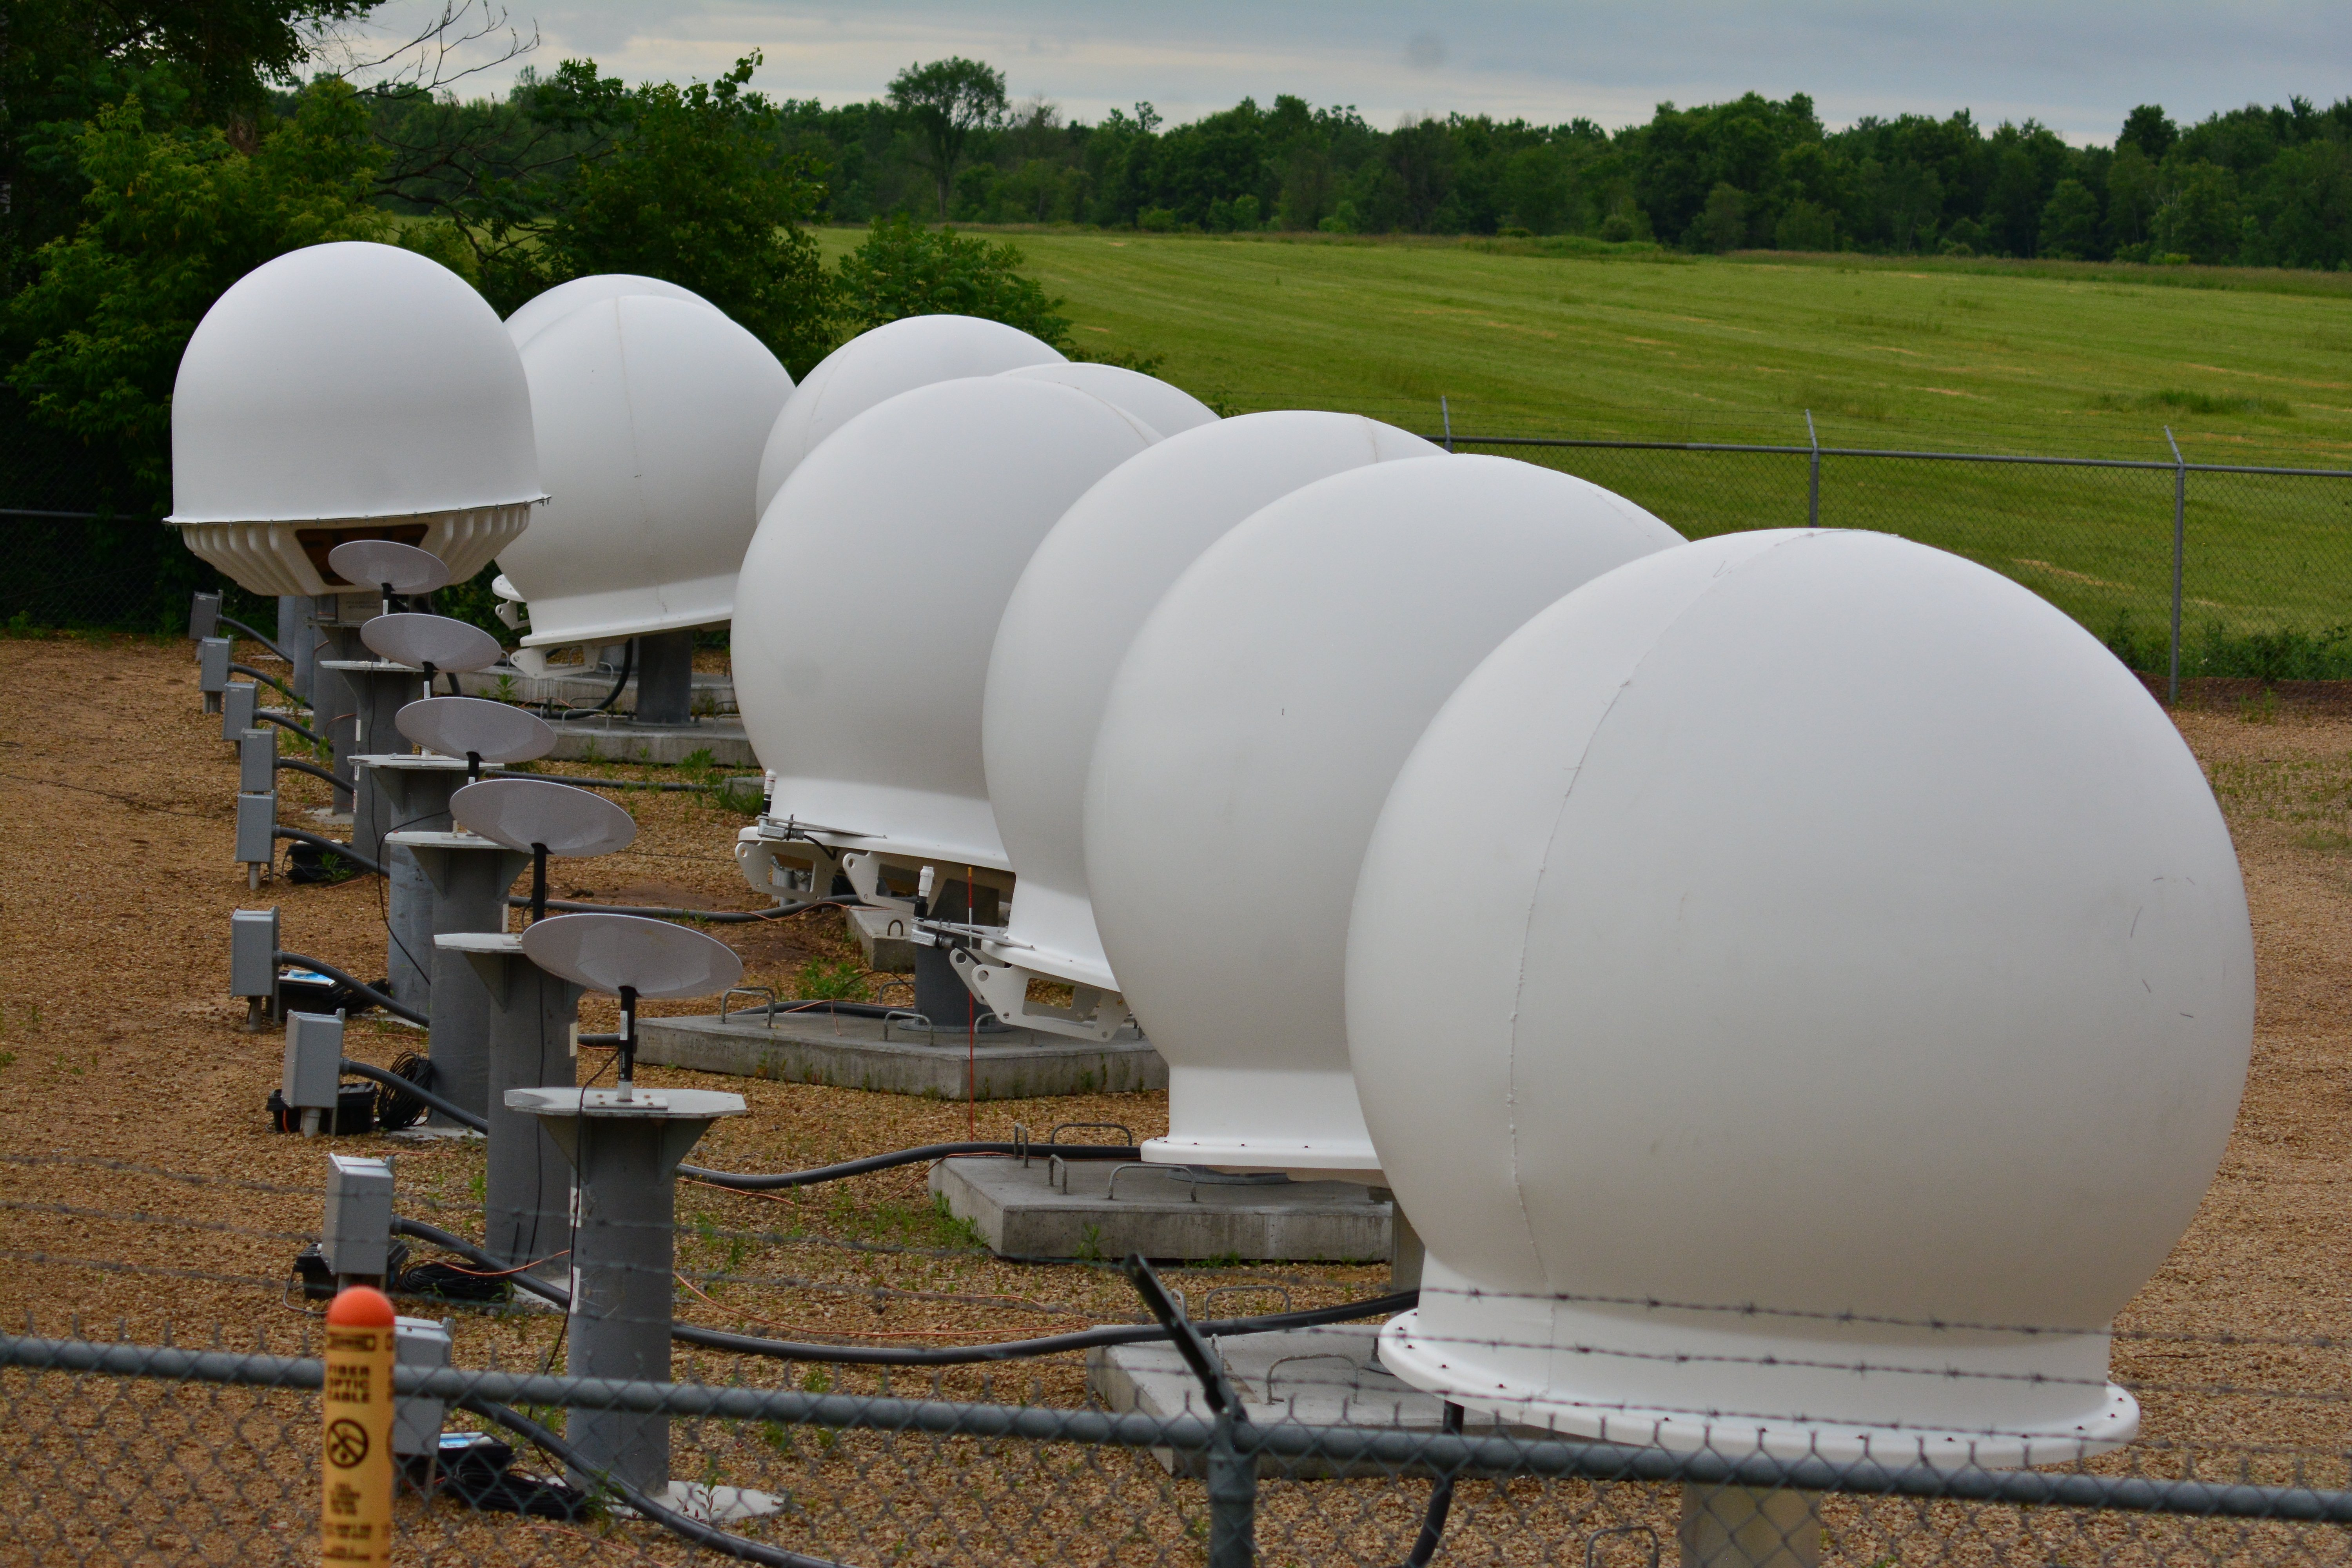
\includegraphics[width=0.6\columnwidth]{img/ground-station.jpeg}
    \caption{A sample ground station, from \small\protect\url{https://reddit.com/r/SpaceXLounge/comments/hcf4t5/prototype_starlink_terminal_closeups_merrillan_wi/}}
    \label{fig:gs}
\end{figure}
    
\begin{figure}
    \centering
    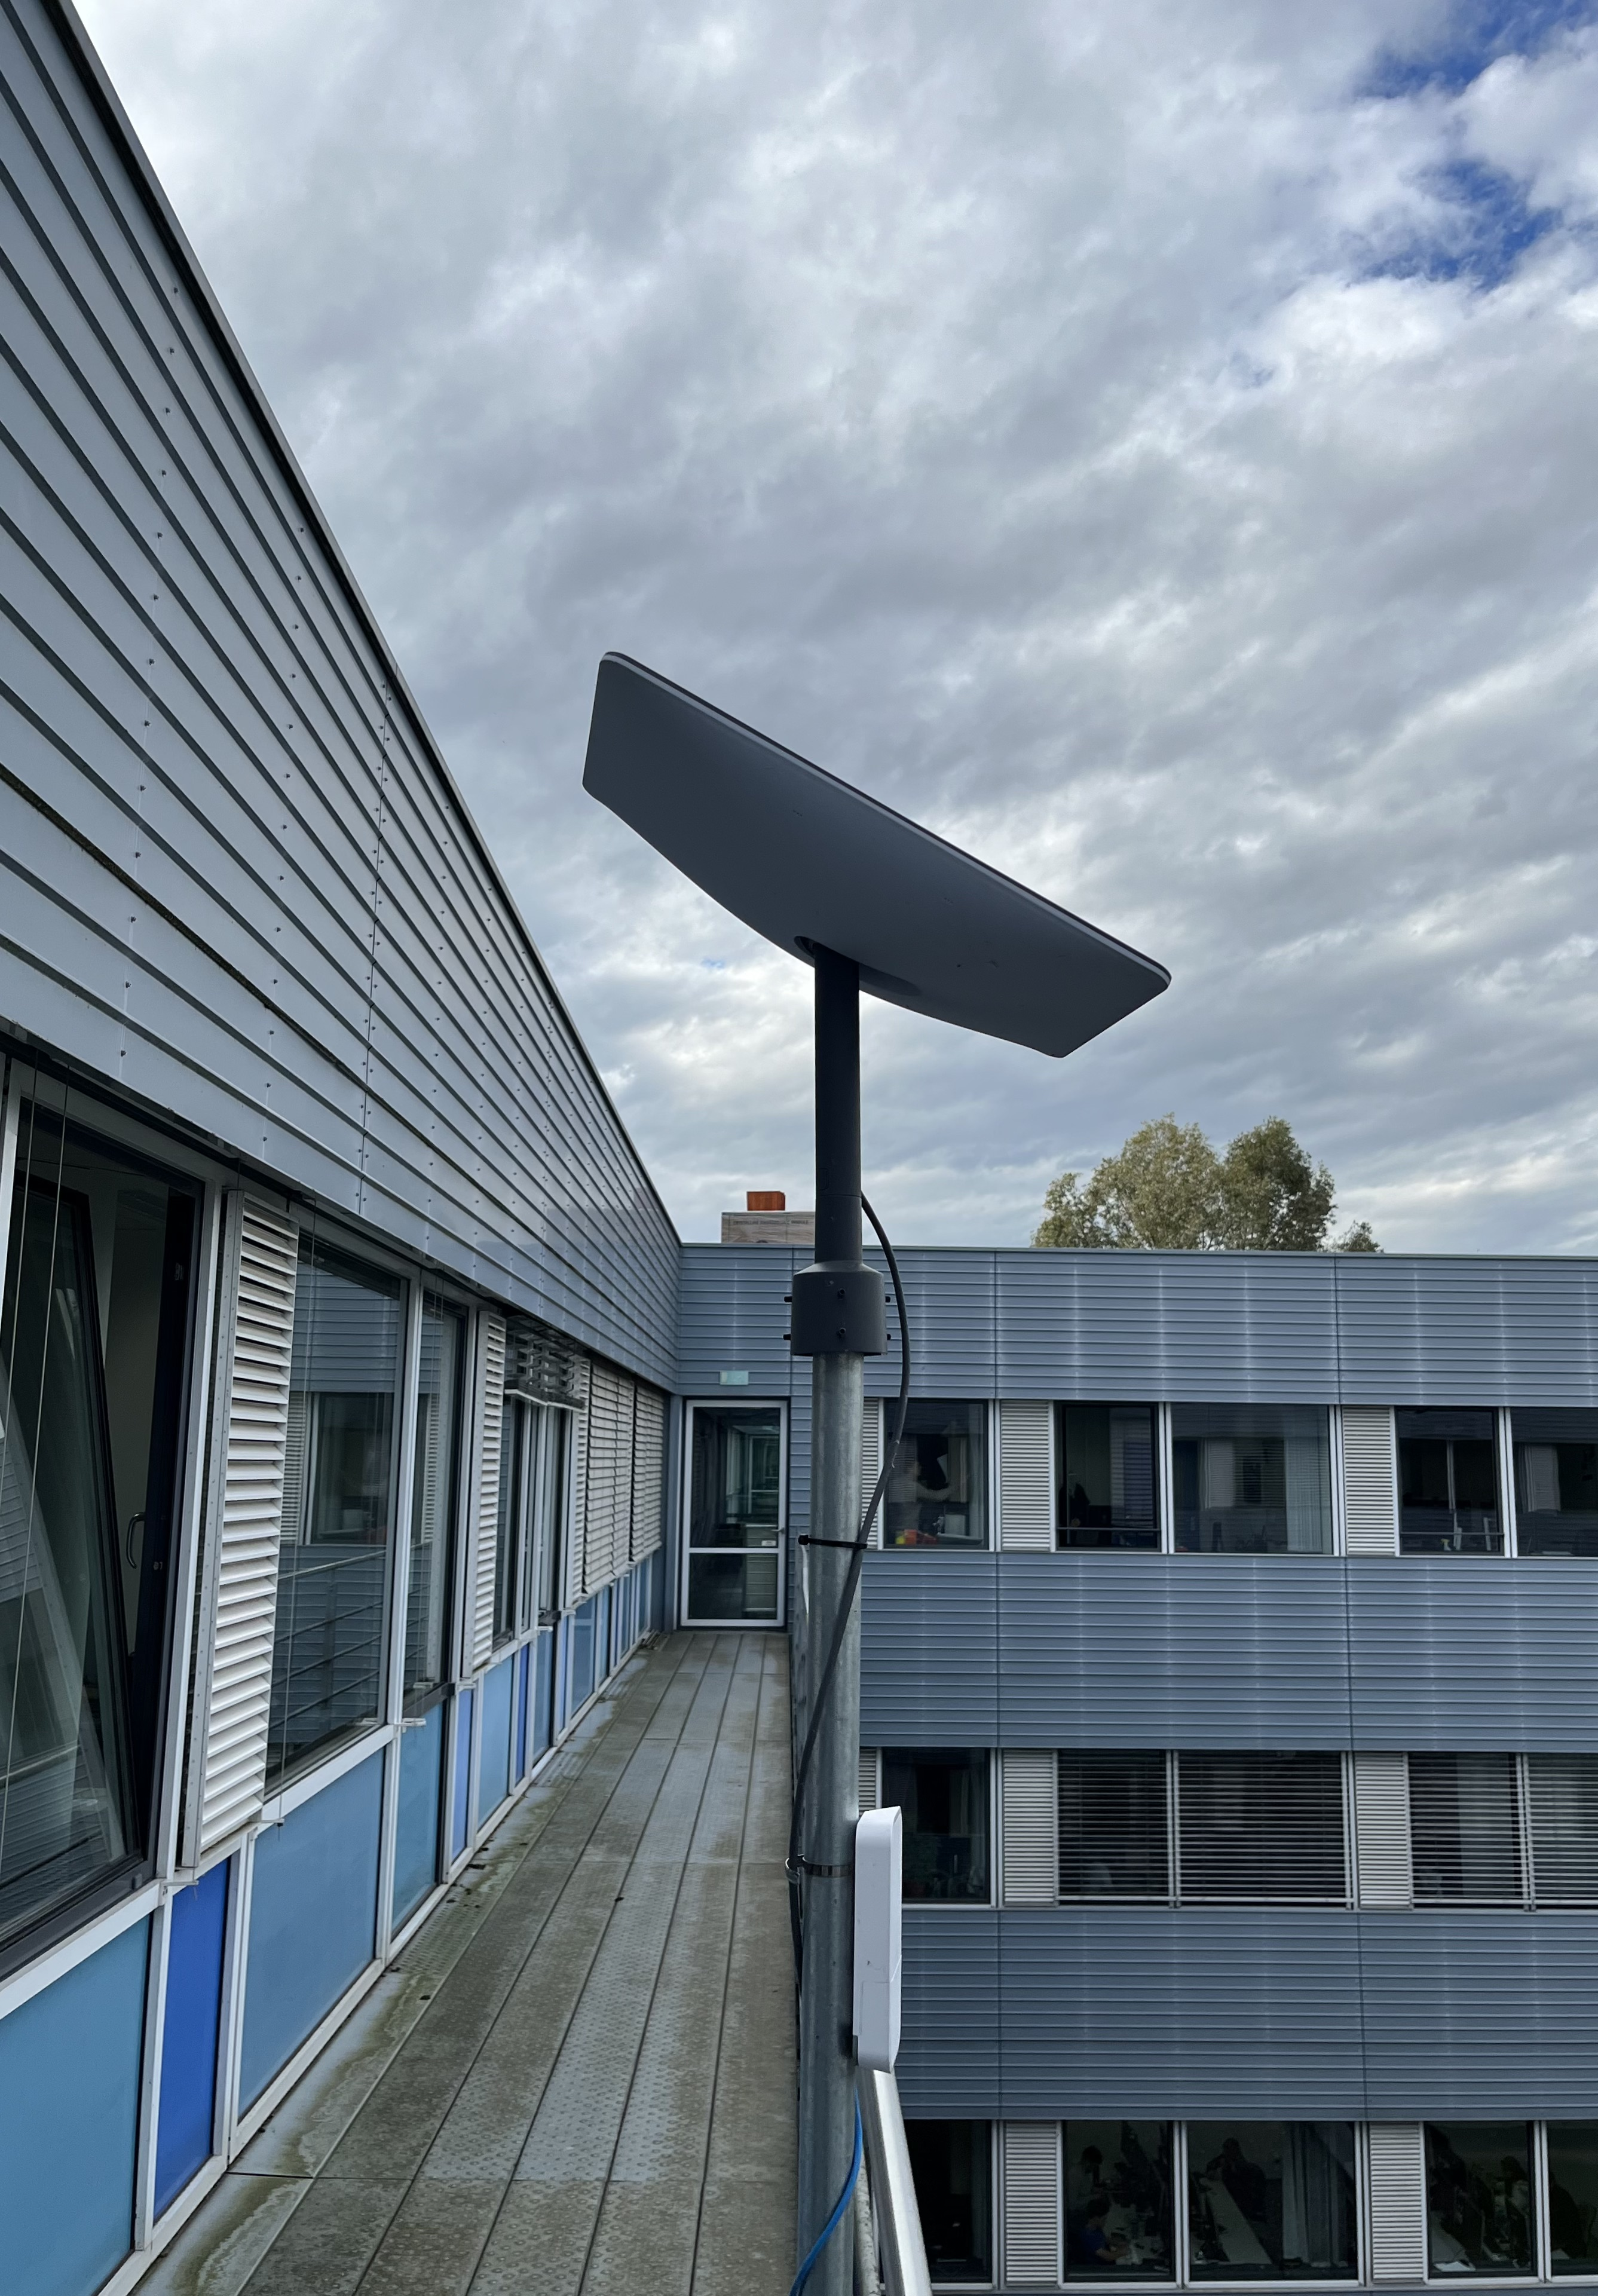
\includegraphics[width=0.6\columnwidth]{img/dish.jpeg}
    \caption{Our Starlink dish, located in Garching, München, DE}
    \label{fig:dish}
\end{figure}
    
\begin{figure}
    \centering
    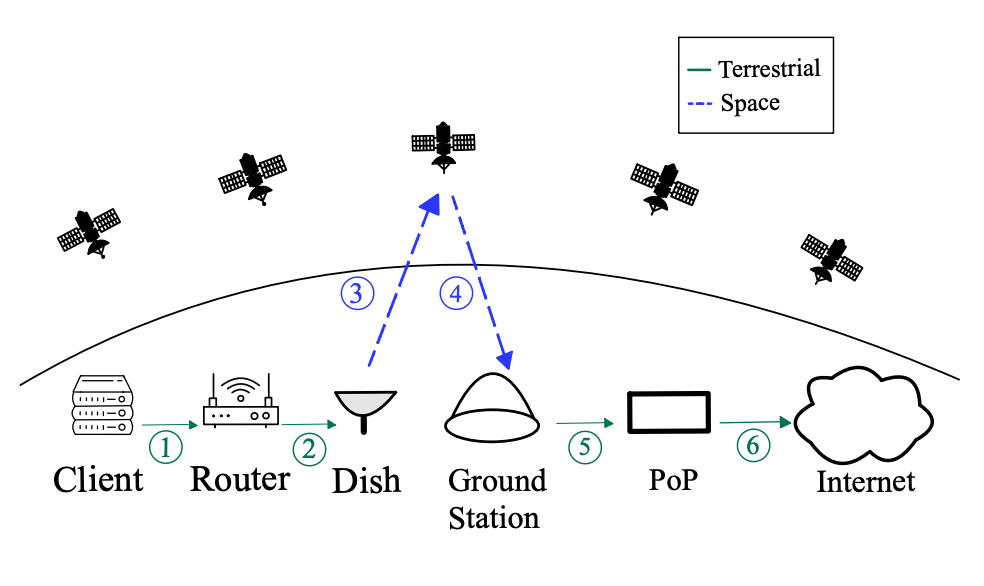
\includegraphics[width=0.6\columnwidth]{img/starlink-101.png}
    \caption{Basic Starlink working, from \cite{izhikevich2023democratizing}}
    \label{fig:starlink-101}
\end{figure}      
    
SpaceX is currently the most popular LEO-based Internet Service Provider. However, other similar projects exist, such as
OneWeb\footnote{\url{https://oneweb.net}} and Amazon Project
Kuiper\footnote{\url{https://aboutamazon.com/what-we-do/devices-services/project-kuiper}}. The former is more enterprise
and government-focused, while the latter aims to be a Starlink competitor, with the first satellite launches starting
now.

The future is bright for LEO-based ISPs; however, we might soon encounter some problems. Starlink alone has currently
4974\footnote{\url{https://celestrak.org/NORAD/elements/gp.php?GROUP=starlink &FORMAT=tle}} satellites in orbit, and
Project Kuiper plans to launch
3236\footnote{\url{https://www.aboutamazon.com/what-we-do/devices-services/project-kuiper}}; these two constellations
alone account for more than 8000 satellites. This is increasing the overall brightness of the skies, and debris
proliferation will become more and more of a concern, as reported by Barentine et al. \cite{cite-key}
    
\section{Background}

We will now introduce some concepts we will use later. We briefly describe the gRPC protocol, as it is used by the dish
to communicate diagnostics and statistics to customers, before describing Two Line Element Sets, the data format used to
encode the satellite's positions. 

For the measurement parts, we are using standard Unix tools, like \texttt{ping}, \texttt{traceroute}, \texttt{iperf},
and we are working with Python for scripting purposes.

\subsection{gRPC protocol}
    
gRPC is an RPC (Remote Procedure Call) framework from Google\footnote{\url{https://grpc.io}}. It is the dish API's
protocol and is massively employed across different fields, especially in microservices architectures. 
    
gRPC uses protocol buffers (protobufs) both as Interface Definition Language and as the format for message interchange;
consequently, every client needs to have a stub providing the server's accessible methods. Typically this involves
generating some \texttt{.proto} files (stubs), but an alternative approach called \textit{Server Reflection}
\footnote{\url{https://github.com/grpc/grpc/blob/master/doc/server-reflection.md}} is employed. With Server Reflection,
it is possible to dynamically query the API to retrieve a list of the accessible methods.

Using a tool like \texttt{grpcurl}\footnote{\url{https://github.com/fullstorydev/grpcurl}}, it is possible to inspect
the service; furthermore, it is easy to use the gRPC python library\footnote{\url{https://pypi.org/project/grpc/}} to
develop scripts.
    
\subsection{Two-line Element Sets}
    
Two-line Element Sets (TLEs) is a widely used ASCII-based data format to encode the position of orbital elements for a
given point in time\footnote{\url{https://en.wikipedia.org/wiki/Two-line_element_set}}. We work with TLEs using the
Skyfield Library\footnote{\url{https://rhodesmill.org/skyfield/}}, an elegant astronomy library for Python. Check
Appendix \ref{app:sky} for a sample script to localize a satellite's position given the Satellite Name. A complete list
of Starlink satellite names can be found at \url{https://celestrak.org/NORAD/elements/gp.php?GROUP=starlink}. 
SATNAME is a unique identifier.
    
Knowing a satellite's position at any given time is a very powerful mechanisms, which allows us to restrict the subset
of satellites the dish may be connected to. It is worth noting that previously, it was possible to call the
\texttt{dish\_get\_context} or similar methods on the API to retrieve such information, as reported by this Reddit
user\footnote{\url{https://reddit.com/r/Starlink/comments/p84o5i/comment/h9o1elp/}}. Unfortunately, these methods now
either return a \texttt{PermissionDenied} error or are deprecated.
    
\begin{lstlisting}[caption={TLE for satellite STARLINK-1007 },captionpos=b]
STARLINK-1007           
1 44713U 19074A   23239.65120160  .00022666  00000+0  15354-2 0  9991
2 44713  53.0553  19.2809 0001296  68.3392 291.7735 15.06406564209327
\end{lstlisting}
    
\section{Related work}
    
Being Starlink a novel technology the existing body of research is somewhat limited, but papers and tools
\footnote{\url{https://github.com/danopstech/starlink\_exporter},\url{https://github.com/sparky8512/starlink-grpc-tools}}
are in development. We created some scripts to work with the dish and to perform some measurements, they are
availableint very same repository that contains this
report\footnote{\url{https://gitlab.lrz.de/netintum/teaching/tumi8-theses/idp-castellotti}}.
    
From a research perspective, different works provide more insights into Starlink — papers like \cite{pan2023measuring}
focus on describing the infrastructure Starlink uses. In contrast, Izhikevich et al. \cite{izhikevich2023democratizing}
illustrate a novel approach to make measurements simpler and cheaper, and Kassem et al.\cite{browser-side} focuses on
running some client-side measurements with a browser extension.
    
Recent work has been carried out on the hardware side, by Wouters \cite{glitching} while Ramponi \cite{quarkslab}
focuses on the firmware perspective and offered valuable insights into the gRPC API.
    
\section{gRPC API}
    
Our first approach to the dish is through the web UI reachable at 192.168.100.1; we discover it is getting data from a
gRPC API running directly on the dish, so we decide to spend some time documenting the available methods we could later
use to gather useful additional information.
    
The server-reflected gRPC API is running on the dish; we can access it by querying it at \texttt{192.168.100.1:9200}
using \texttt{grpcurl}\footnote{\url{https://github.com/fullstorydev/grpcurl}}, a sample query to retrieve downlink
throughput is:
    
\begin{lstlisting}[language=bash]
rc@gnolmir:~$ grpcurl -plaintext -d '{"get_status":{}}' 192.168.100.1:9200 SpaceX.API.Device.Device/Handle
{
    "apiVersion": "10",
    ... (output omitted)
}
\end{lstlisting}

It is then possible to use \texttt{jq} to extract the needed fields. We can use the following command to describe the
available services:
    
\begin{lstlisting}[language=bash]
rc@gnolmir:~$ grpcurl -plaintext 192.168.100.1:9200 describe
SpaceX.API.Device.Device is a service:
service Device {
    rpc Handle ( .SpaceX.API.Device.Request ) returns ( .SpaceX.API.Device.Response );
    rpc Stream ( stream .SpaceX.API.Device.ToDevice ) returns ( stream .SpaceX.API.Device.FromDevice );
}
grpc.reflection.v1alpha.ServerReflection is a service:
service ServerReflection {
    rpc ServerReflectionInfo ( stream .grpc.reflection.v1alpha.ServerReflectionRequest ) returns ( stream .grpc.reflection.v1alpha.ServerReflectionResponse );
}
\end{lstlisting}
    
Then, describe the single service using the following:
    
\begin{lstlisting}[language=bash]
rc@gnolmir:~$ grpcurl -plaintext 192.168.100.1:9200 describe SpaceX.API.Device.Request
SpaceX.API.Device.Request is a message:
message Request {
    uint64 id = 1;
    string target_id = 13;
    uint64 epoch_id = 14;
    oneof request {
    .SpaceX.API.Device.SignedData signed_request = 15;
    .SpaceX.API.Device.RebootRequest reboot = 1001;
    .SpaceX.API.Device.SpeedTestRequest speed_test = 1003;
    ... (output omitted)
    }
\end{lstlisting}
    
Here\footnote{\url{https://gist.github.com/rcastellotti/e20630366dfeaeada6cc2680f562f6ac}} is a complete list of
available methods as of September 2023.

To simplify scripting, we develop a simple wrapper library around the gRPC API
\footnote{\url{https://gitlab.lrz.de/netintum/teaching/tumi8-theses/idp-castellotti/-/blob/main/api.py}} and a CLI
tool\footnote{\url{https://gitlab.lrz.de/netintum/teaching/tumi8-theses/idp-castellotti/-/blob/main/s.py}} to use the
library in command line. It should be trivial to add functionality to the library.

Unlike \texttt{sparky8512/starlink-grpc-tools}, we do not make any assumptions about the format used to save data.

After having laid the groundwork to understand the next section, we now move to the measurements we performed.
    
\chapter{Measurements and Analysis}

After getting acquainted with our working environment, we run several measurements to better understand Starlink internals. 
    
We first try to understand the possible differences in package routing between Starlink-based and default cabled
connections. We then move to measure the latency and bandwidth of links, and we check whether the values for bandwidth
reported from the API are the same as our machine reports. Later, we will try to understand whether we can spot physical
layer influences on the latency of connections.  
    
In the second part of our measurements, we explore the satellite part of the infrastructure. First, we implement tooling
to identify satellites in line of sight of our dish and to detect patterns in satellite appearances before implementing
a side-channel measurement to detect satellite handovers based on the approach Izhikevich's approach
\cite{izhikevich2023democratizing}.
    
\section{Routing}
    
In this section, we delve into the exploration of the routing behavior in Starlink-based connections; routing refers to
the process of selecting a path across one or more
networks\footnote{\url{https://www.cloudflare.com/learning/network-layer/what-is-routing/}}. To investigate such topic,
we use traceroutes; \texttt{traceroute (8)}  is a tool used to diagnose problems in a network path; it is used to
understand the path IP packets are taking from one computer (source IP address) to another (destination IP address).

One of the first experiments we perform is running traceroutes to several different geographically sparse targets; we
retrieve a list of those from major cloud vendors,\footnote{\url{ https://gstatic.com/ipranges/cloud.json},
\url{https://ip-ranges.amazonaws.com/ip-ranges.json}, \url{https://microsoft.com/en-us/download/details.aspx?id=53601}},
\footnote{\url{https://docs.oracle.com/en-us/iaas/tools/public_ip_ranges.json }}. We are both using the
\texttt{traceroute (8)} standard UNIX tool and a custom python
script\footnote{\url{https://gitlab.lrz.de/netintum/teaching/tumi8-theses/idp-castellotti/-/blob/main/cloud-traceroutes.py}}
to run traceroutes and save data to CSV files.
    
We carefully select our target destinations from major cloud vendors. The reason behind this selection is that these
cloud vendors publish their IP ranges, and their host locations are known. While the precise location of the final
target in complex networks remains challenging to assess, the last hop in a traceroute often provides a reasonably
accurate approximation. It is worth noting that in private networks, the hosts often do not respond to ICMP pings,
further obscuring the packet's route.

We run the traceroutes using ICMP, UDP, and TCP protocols using both the Starlink and the default network interface over
several days, and we save the results to CSV files. Subsequently, we use NetworkX, a Python package for the creation,
manipulation, and study of the structure, dynamics, and functions of complex
networks\footnote{\url{https://networkx.org/}}. to visualize whether we can spot some differences in the graphs we
create. 
The following Figures are some of the representations for traceroutes to certain specific hosts. While running
traceroutes, it is common to retrieve information for the first 30 hops; however, we decided to limit ourselves to the
first seven hops because we do not receive answers for further hops. 

\begin{figure}
    \label{fig:tr_aws_icmp}
    \centering
    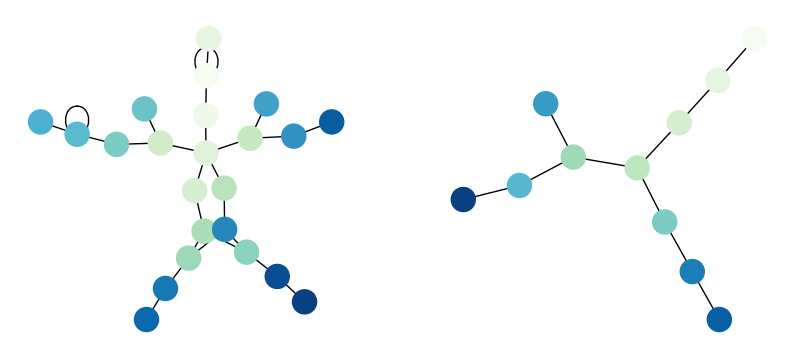
\includegraphics[width=0.6\columnwidth]{img/tr_aws_icmp.png}
    \caption{Visualizing traceroutes to 4 different hosts from AWS using ICMP, the left Figure refers to Starlink traceroutes; the right one is the cabled network interface.}
\end{figure}
    
\begin{figure}
    \label{fig:tr_aws_udp}
    \centering
    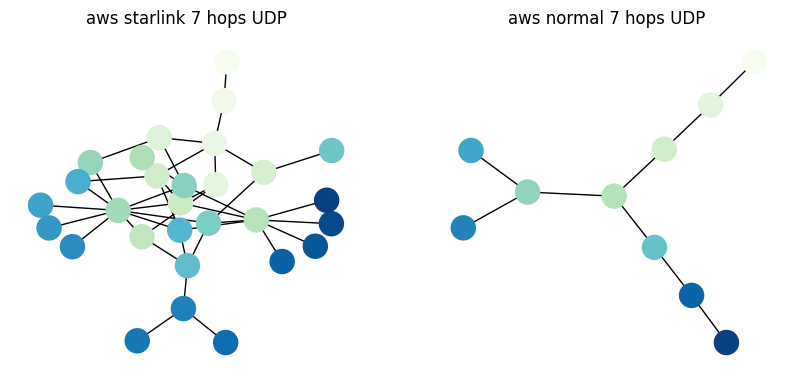
\includegraphics[width=0.6\columnwidth]{img/tr_aws_udp.png}
    \caption{Visualizing traceroutes to 4 different hosts from AWS using UDP, the left Figure refers to Starlink traceroutes; the right is the cabled network interface.}
\end{figure}
    
\begin{figure}
    \label{fig:tr_aws_tcp}
    \centering
    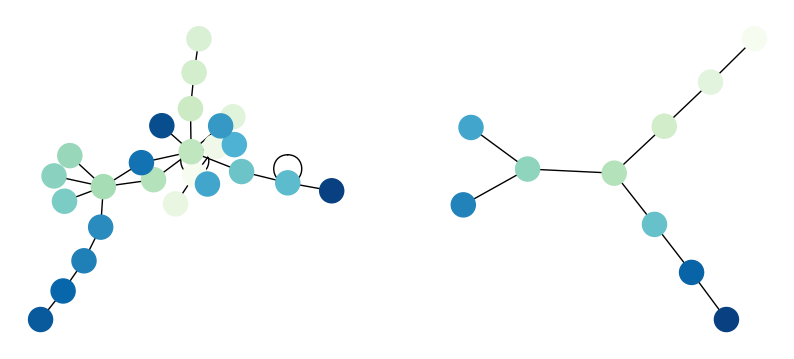
\includegraphics[width=0.6\columnwidth]{img/tr_aws_tcp.png}
    \caption{Visualizing traceroutes to 4 different hosts from AWS using TCP, the left Figure refers to Starlink traceroutes; the right is the cabled network interface.}
\end{figure}
    
\begin{figure}
    \label{fig:tr_azure_icmp}
    \centering
    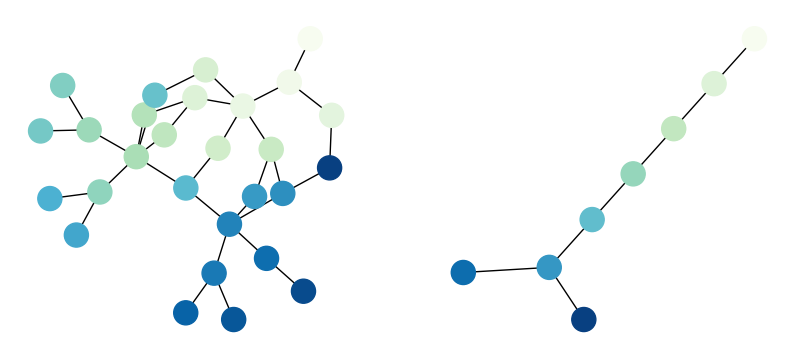
\includegraphics[width=0.6\columnwidth]{img/tr_azure_icmp.png}
    \caption{Visualizing traceroutes to 4 different hosts from Azure using ICMP, the left Figure refers to Starlink traceroutes, the right one is the default network interface.}
\end{figure}
    
Upon analyzing the traceroute data, it is evident that the routing within the Starlink network exhibits a notably higher
degree of complexity compared to the cabled ISP network traceroutes. While the default traceroutes show data following
relatively straightforward paths in four different main directions, the Starlink traceroutes display a more intricate
and convoluted routing pattern. Several factors could contribute to this complexity, including diverse routing decisions
and the possibility of Inter Satellite Routing within the Starlink constellation.

We are only reporting traceroutes to AWS using the three most common methods and a traceroute to Azure; more data to
visualize can be found in the accompanying
repository\footnote{\url{https://gitlab.lrz.de/netintum/teaching/tumi8-theses/idp-castellotti-data}}.
    
We do not find any significant differences comparing traceroutes over different days; we see hops in the same Autonomous
Systems; the only difference we are able to observe is that we reach different hosts inside AS14593, the Autonomous
System SpaceX operates\footnote{\url{https://bgp.he.net/AS14593}}.
    
Table \ref{tab:hops} contains a list of hosts reached together and a count of how many times we reached the target.
    
\begin{table}
    \label{tab:hops}
    \centering
    \begin{tabular}{ r r }
        \toprule
            host           & count \\ 
            \midrule
            206.224.65.204 & 595   \\
            206.224.65.200 & 595   \\
            206.224.65.208 & 549   \\ 
            206.224.65.182 & 444   \\
            206.224.65.196 & 440   \\ 
            206.224.65.188 & 360   \\ 
            206.224.65.129 & 358   \\ 
            206.224.65.178 & 274   \\ 
            206.224.65.180 & 235   \\ 
            206.224.65.184 & 189   \\ 
            206.224.65.186 & 159   \\ 
            206.224.65.190 & 151   \\
            \bottomrule
    \end{tabular}
    \caption{Targets reached inside AS14593 together with the count}
\end{table}

We also see some different prefixes in later traceroutes; AS14593 advertises
many\footnote{\url{https://bgp.he.net/AS14593\#_prefixes}}.
    
\section{Latency Analysis}

The gRPC API exposes a \texttt{get\_status} method containing a \texttt{pop\_ping\_latency\_ms} field, so we decide to
measure the stability of latency to the Point of Presence (PoP) -- an artificial demarcation point or network interface
point between communicating entities. A common example is an ISP point of presence, the local access point that allows
users to connect to the Internet with their Internet service provider
(ISP)\footnote{\url{https://en.wikipedia.org/wiki/Point_of_presence},
\url{https://networkencyclopedia.com/point-of-presence-pop/}}.

We know that in AS14593, there are several geographically distributed hosts containing "pop" in their hostname, such as
\texttt{customer.dnvrcox1.pop.starlinkisp.net}, the naming scheme suggests the position of the PoP we are analyzing, in
the previous example it is located in Denver, Colorado.
Here\footnote{\url{https://gitlab.lrz.de/netintum/teaching/tumi8-theses/idp-castellotti-data/-/blob/main/pops.json}} is
a brief list of different PoPs retrieved using censys\footnote{\url{https://search.censys.io/}}.

Latency, defined as the time it takes for data to pass from one point on a network to
another\footnote{\url{https://www.cloudflare.com/learning/performance/glossary/what-is-latency/}}, to the PoP is pretty
stable, as SpaceX reports it fluctuates around 35 milliseconds, as we can verify from Figure \ref{fig:vis-latency}. We
are not able to observe any patterns in latency fluctuation.

\begin{figure}
    \centering
    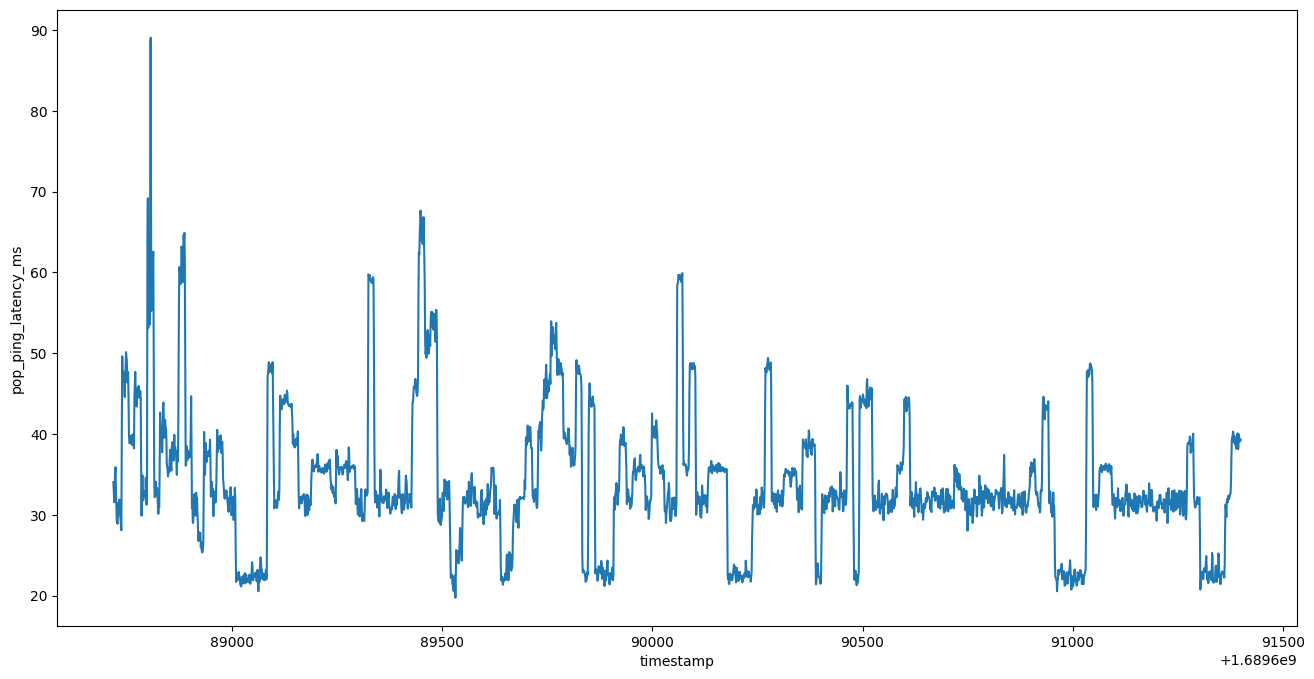
\includegraphics[width=1\columnwidth]{img/latency.png}
    \caption{Visualizing latency to the Point of Presence.}
    \label{fig:vis-latency}
\end{figure}

\section{Bandwidth analysis}

During our investigations, we analyze bandwidth for two reasons: first, we want to check whether the data from the API
was correct, and then we want to see whether we can detect any patterns in bandwidth drops.

The first experiment we set up is the following: We start downloading five Debian ISOs from different mirrors (to
neutralize the effect of the single upload speed of a mirror). While downloading the files, we are also running a script
to extract downlink throughput from the dish and measuring it simply by getting data from
\path{/sys/class/net/{interface}/statistics/rx_bytes} in order to compare the data reported from the API and the actual
bandwidth our machine reports.

Figure \ref{fig:vis-bw-15sec} shows our results, \texttt{bandwidth\_bps} is the data we obtain from
\path{/sys/class/net/{interface}/statistics/rx_bytes}, while \texttt{downlink\_throughput\_bps} is the data reported
from the gRPC API. As the data reports, the two values are very similar; this suggests that the dish reports bandwidth
correctly.

From \cite{llc-application}, we know the dish seeks better connections, as satellites move constantly, every 15 seconds.
We plot vertical lines every 15 seconds and shift them to detect whether the bandwidth drops were happening in 15-second
intervals.

\begin{figure}
    \centering
    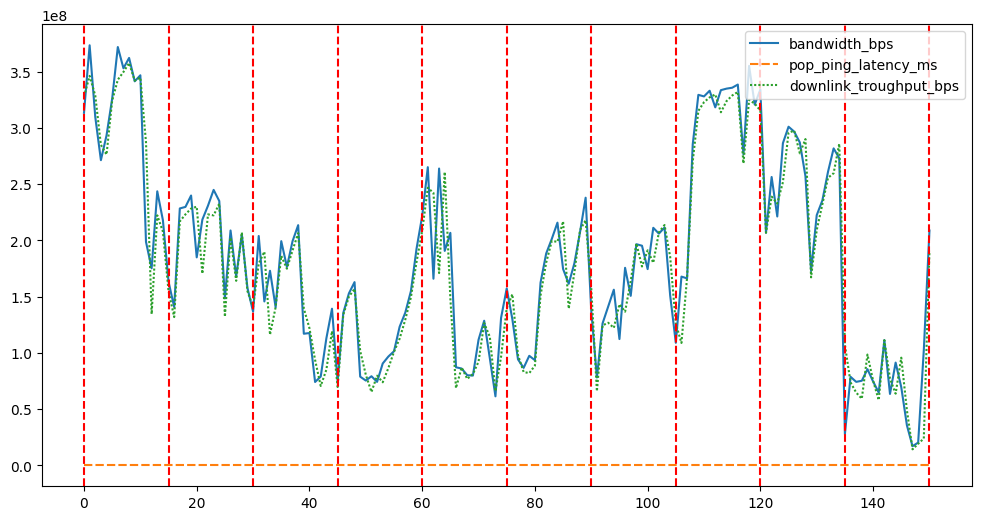
\includegraphics[width=1.0\columnwidth]{img/bw-15seconds.png}
    \caption{Bandwidth visualization, with vertical red lines every 15 seconds.}
    \label{fig:vis-bw-15sec}
\end{figure}

We repeat the experiments by shifting the red vertical lines and changing the intervals for collected data, and in the
majority of cases, we see that whenever we draw a vertical red line, we have some drop in the immediate milliseconds
before or after; however, drops also happen in different intervals. Initially we thought these drops might be related to
satellite handovers, so we investigated further; check Section \ref{sec:sat-hand-drop}, where we investigate the
correlation between satellite handovers (retrieved using a side-channel) and drops in bandwidth. 

\section{Physical layer influences on latency}

After measuring latency and bandwidth and noticing some drops in semi-regular intervals, we decided to investigate
whether the physical layer has any influences on latency in some way. Our intuition is that if this is the case, we can
approximately detect whether a certain amount of data is needed before a packet is sent; this means in the \textbf{best-case
scenario} we send the packet we want to reach the Internet exactly, it fills exactly the size window and it is sent
immediately, \textbf{worst-case scenario} we sent the packet when the previous packet was just sent and we need to wait to fill
the window before sending the packet. Of course, this operation introduces some performance drawbacks in the worst-case
scenario, as the dish might have to delay transmission to wait for more data.

To verify this hypothesis, we try to send some payload with iPerf\footnote{\url{https://iperf.fr/}} on the network
interface used by Starlink. We send payloads of increasing sizes (10k, 20k, 50k, 100k, 1M, 10M) and measure the RTT. 
Figure \ref{fig:rtt-iperf} contains a visualization, as we can notice background traffic has no impact on performance.
\begin{figure}
    \label{fig:rtt-iperf}
    \centering
    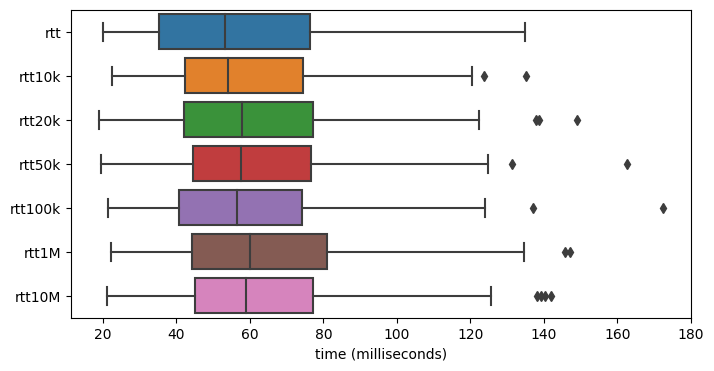
\includegraphics[width=0.6\columnwidth]{img/latency_iperf.png}
    \caption{Latency variation while sending traffic on the uplink using iPerf}
\end{figure}

We conclude no such mechanism is enabled on the device, it might be possible other smarter and better technologies are
employed and they operate at the ideal point and thus are hard to detect.

\section{Visible Satellites}

One of the first measurements we perform with satellites is to retrieve the subset of satellites the dish might be
connected to.

It is up to us to define what "visible" means; in our evaluations, we decide that, knowing the satellites orbit around
Earth at around 550 kilometers, it is reasonable to assume a satellite is visible when it is above the horizon and it is
(point to point) not further away than 800 kilometers. The ground truth might be different, but this approximation
allows us to formulate and hypothesis around satellites positions. 

The first measurement we set up is the following: every 15 seconds, we run a script that retrieves all the visible
satellites and stores them in a SQLite database. If we see the same satellite in the iteration before we update the
\texttt{timestamp} otherwise, we create a new row in the database. We use a \texttt{relative\_ts} (relative timestamp)
to enumerate every measurement (a probe every 15 seconds). To measure visible satellites, we are using the
\texttt{common.calculate\_visible\_satellites} function using Garching coordinates as latitude and longitude parameters
and a distance of 800 Kms. The script can be found in Listing \ref{lst:cvs}.

After collecting data for several hours, we plot satellite appearances to check whether their appearance is following
some pattern; Figure \ref{fig:vis-sat-pat} reveals this is the case; we are able to observe the same satellites every 12
hours roughly. For some satellites, we notice some artifacts that might induce to think there is a change in the
pattern, but this is not true; the interval between the appearances is the same as in the other cases; we are uncertain
about the reasons we are seeing this phenomenon.

\begin{figure}
    \centering
    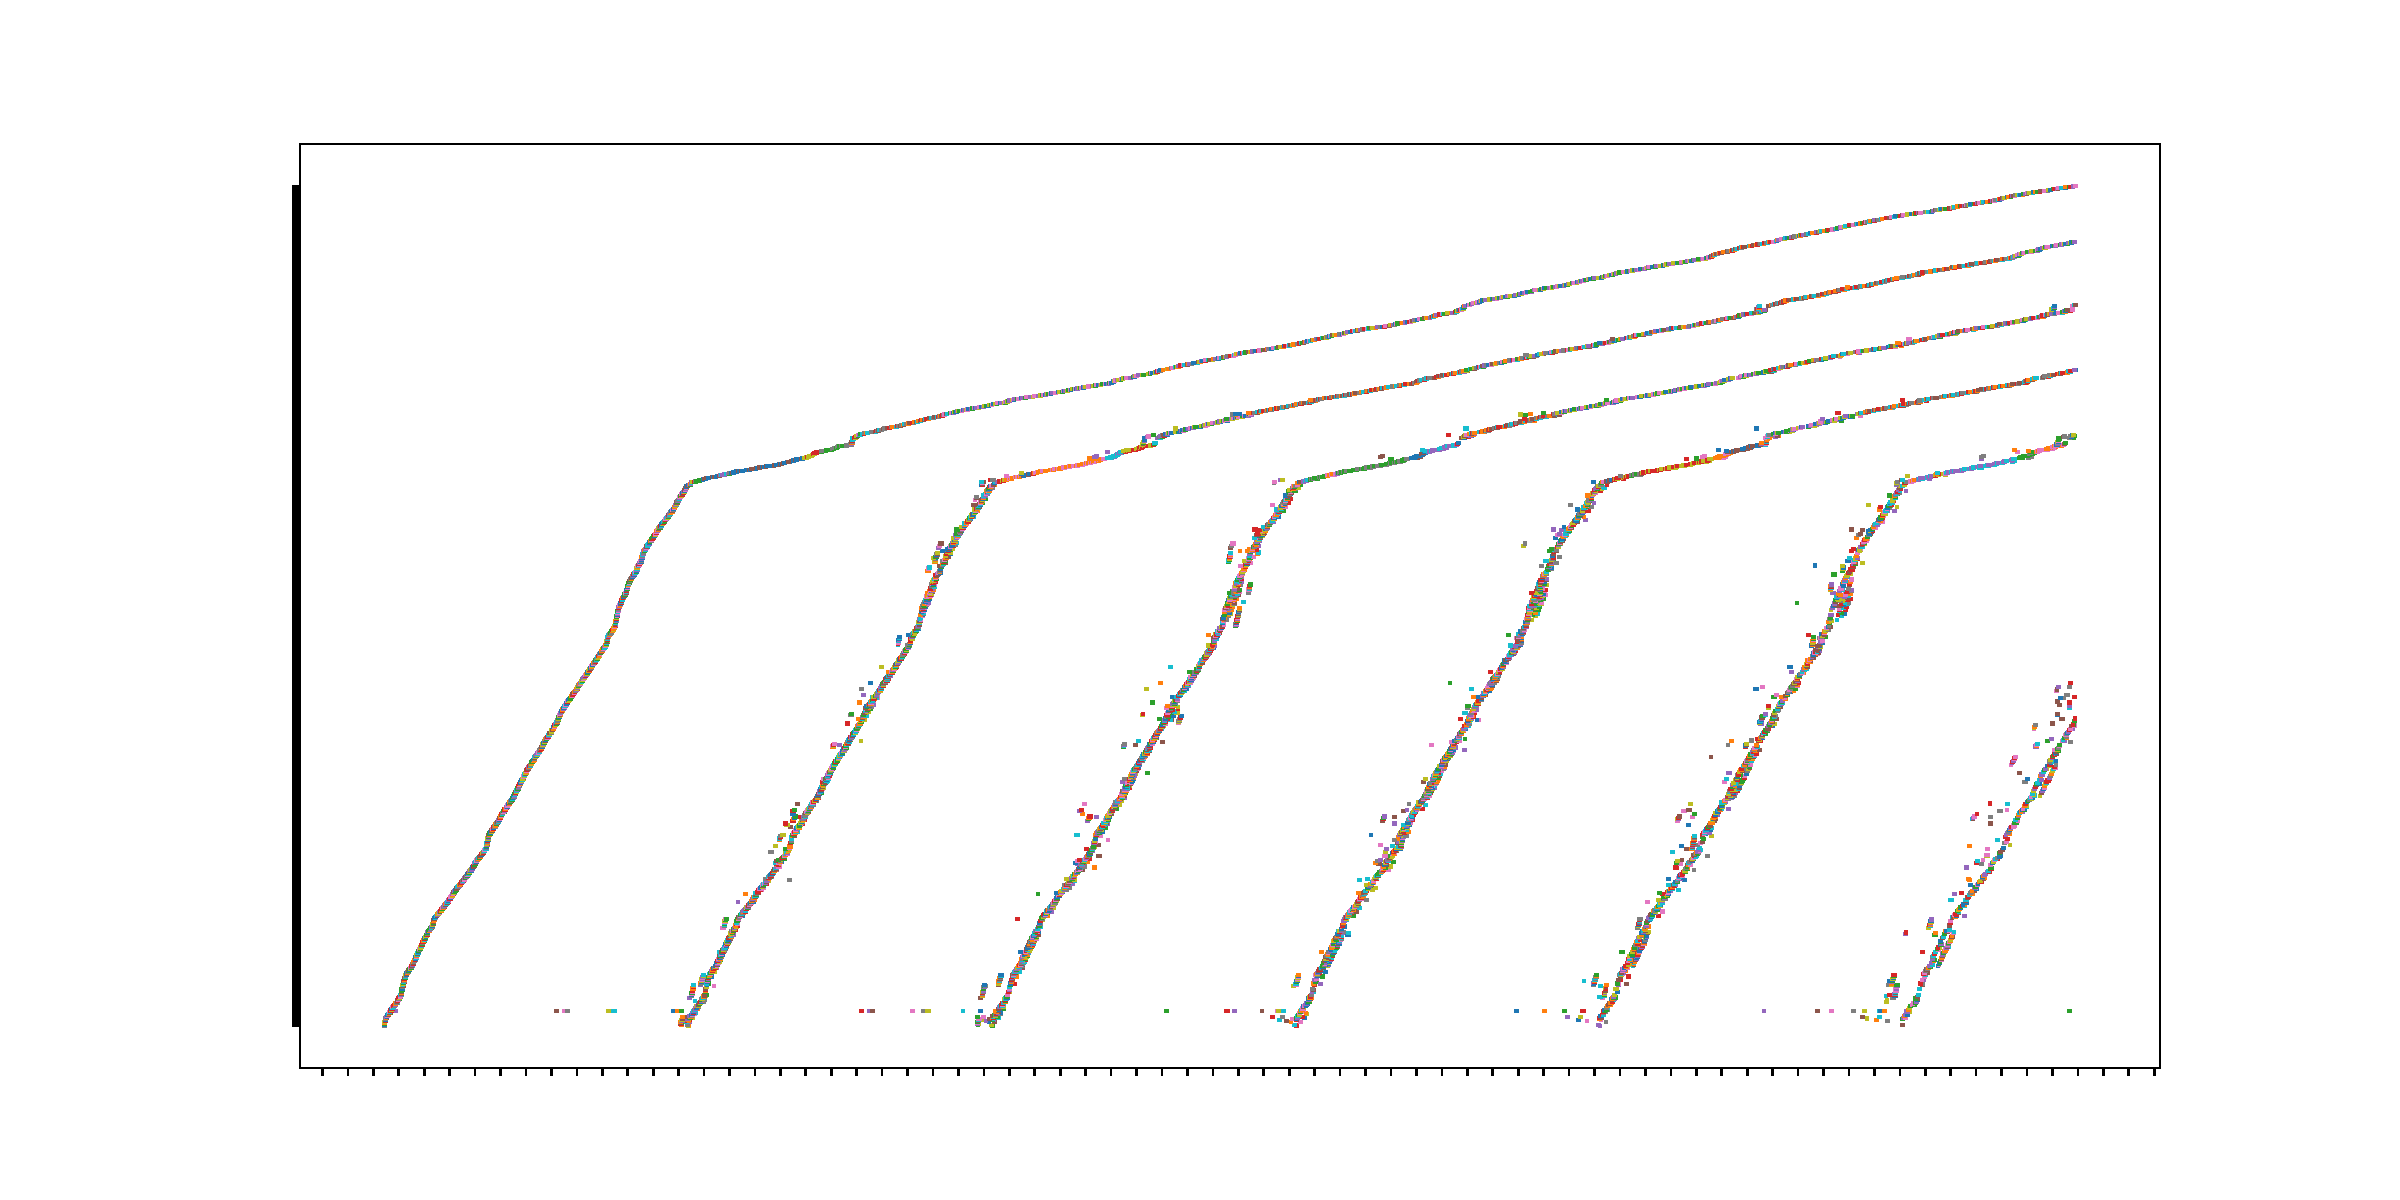
\includegraphics[width=1.0\columnwidth]{img/patterns-in-satellite-appearances.pdf}
    \caption{Visualizing patterns in satellite appearances, we roughly see the same satellite every 12 hours.}
    \label{fig:vis-sat-pat}
\end{figure}

\section{Detecting Satellite Handovers}

Unfortunately, as mentioned earlier, it is impossible to know from the gRPC API which satellite the dish is connected to.

The Starlink gRPC API, however, exposes a \texttt{dish\_get\_obstruction\_map} method. Following the approach described
in Izhikevich's paper \cite{izhikevich2023democratizing}, we use the information gathered from polling the endpoint each
second to extract the current obstruction map and visualize satellite handovers. This works because the dish adds a dot
(setting a value to 1) in a 123*123 matrix whenever it sees a satellite in that position. 

The matrix is cleared whenever the dish is rebooted by setting every entry to -1; whenever a satellite is detected, the
entry is set to 1. 

By polling the endpoint frequently enough, we can observe satellite traces, and by comparing values in the matrices we
obtain, we can detect whether a satellite handover was performed.

Let us assume the following matrices are retrieved at $ t_x $ and $ t_{x+1} $, respectively. 
In the first matrix, we have ones in $ (0,2) $ and $ (1,3) $; in the second one, we have ones in $ (0,2) $, $ (1,3) $, $
(2,4) $. This means the new satellite we saw at $ t_{x+1} $ is on the same path as the satellites before. Thus, NO
handover was performed. \vspace{10mm}

$\begin{bmatrix}
-1 & -1 & \color{red}1 &           -1 & -1 \\
-1 & -1 &           -1 & \color{red}1 & -1 \\
-1 & -1 &           -1 &           -1 & -1 \\
-1 & -1 &           -1 &           -1 & -1 \\
-1 & -1 &           -1 &           -1 & -1 \\ 
\end{bmatrix}
+
\begin{bmatrix}
-1 & -1 & \color{red}1 &           -1 &           -1 \\
-1 & -1 &           -1 & \color{red}1 &           -1 \\
-1 & -1 &           -1 &           -1 & \color{red}1 \\
-1 & -1 &           -1 &           -1 &           -1 \\
-1 & -1 &           -1 &           -1 &           -1 \\
\end{bmatrix}
=
\begin{bmatrix}
-2 & -2 & 2 &  -2 &           -2 \\
-2 & -2 & -2 &  2 &           -2 \\
-2 & -2 & -2 & -2 & \color{red}0 \\
-2 & -2 & -2 & -2 &            -2 \\
-2 & -2 & -2 & -2 &            -2 \\
\end{bmatrix}$ \vspace{10mm}

In this different case, the new satellite we see at $ t_{x+1} $ is in a different location, so a handover must have been
performed. \vspace{10mm}

$\begin{bmatrix}
-1 & -1 & \color{red}1 &           -1 & -1 \\
-1 & -1 &           -1 & \color{red}1 & -1 \\
-1 & -1 &           -1 &           -1 & -1 \\
-1 & -1 &           -1 &           -1 & -1 \\
-1 & -1 &           -1 &           -1 & -1 \\
\end{bmatrix}
+
\begin{bmatrix}
-1 & -1 & \color{red}1 &           -1 & -1 \\
-1 & -1 &           -1 & \color{red}1 & -1 \\
-1 & -1 &           -1 &           -1 & -1 \\
-1 & -1 &           -1 &           -1 & -1 \\
1 & -1 &            -1 &           -1 & -1 \\
\end{bmatrix}
=
\begin{bmatrix}
          -2 & -2 & 2 & -2 & -2 \\
          -2 & -2 & -2 & 2 & -2 \\
          -2 & -2 & -2 & -2 & -2 \\
          -2 & -2 & -2 & -2 & -2 \\
\color{red}0 & -2 & -2 & -2 & -2 \\
\end{bmatrix}$

\vspace{10mm}

We can observe it is pretty easy to detect whether a handover was performed; it is sufficient to sum the two matrices
and check whether the $ 0 $ value (there was -1 before, and we currently have 1) is near an entry whose value is $ 2 $
(at $ t_{x} $ value was 1, and at $ t_{x+1} $ value is $ 1 $). 

First, we must write a script to extract obstruction maps from the dish. To achieve this goal, we can use the
\texttt{api.get\_obstruction\_map}
\footnote{\url{https://gitlab.lrz.de/netintum/teaching/tumi8-theses/idp-castellotti/-/blob/main/api.py?ref_type=heads\#L54}}
function, which returns a JSON response similar to this:

\begin{lstlisting}[caption={data from the \texttt{dish\_get\_obstruction\_map} function},captionpos=b]

{'apiVersion': '9',
 'dishGetObstructionMap': {'minElevationDeg': 10.0,
                           'numCols': 123,
                           'numRows': 123,
                           'snr': [-1.0,
                                   -1.0,
                                   -1.0,
                                   1.0,
                                   1.0,
                                   -1.0,
                                   -1.0,
                ...,
                                   1.0,
                                   1.0,
                                   1.0,
                                   -1.0,\label{sec:sat-hand-drop}

                                   -1.0,
                                   -1.0,
                                   -1.0]}}  
\end{lstlisting}

We can now extract the values in \texttt{map["dishGetObstructionMap"]["snr"]} and reshape the array in a $123\times123$
with \texttt{np.array(map).reshape(123, 123)}. This allows to visualize the obstruction map at any given moment; it is a
matter of loading the JSON file we want to visualize and plot it with matplotlib \cite{Hunter:2007}, code can be found
in Listing \ref{listing-obs} and the visualization is Figure \ref{fig:vis-single-map}.

\begin{lstlisting}[language=python,caption={visualizing a single obstruction map},captionpos=b,label=listing-obs]
import json
import numpy as np
import matplotlib.pyplot as plt

f = "1692089163.json"
map = json.load(open(f))
map = map["dishGetObstructionMap"]["snr"]
map = np.array(map).reshape(123, 123)
plt.imshow(map)
plt.show()
\end{lstlisting}

\begin{figure}
    \centering
    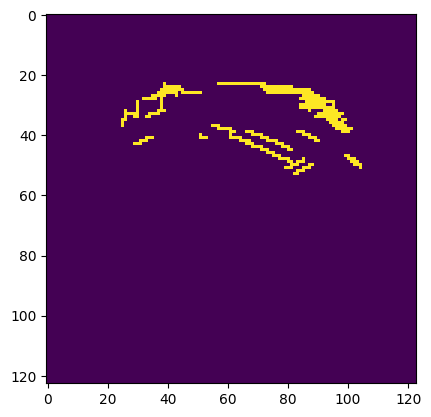
\includegraphics[width=0.5\columnwidth]{img/single_map.png}
    \caption{Visualizing a single obstruction map, satellite traces are clearly visible.}
    \label{fig:vis-single-map}
\end{figure}

Following this approach, we can create a simple script to retrieve maps each second and save them locally; later, we can
export images and create a video to better visualize the phenomenon, we have uploaded a sample video at
\url{https://www.youtube.com/watch?v=PjfMPr20suw}.

\section{Correlating Handovers and Drops in Bandwidth}
\label{sec:sat-hand-drop}

We create a simple script to algorithmically detect handovers; we can use the function
\texttt{common.detect\_handovers}\footnote{\url{https://gitlab.lrz.de/netintum/teaching/tumi8-theses/idp-castellotti/-/blob/main/common.py}}
to detect whether a handover was performed between two subsequent snapshots; getting all the handovers is simply a
matter of iterating for every JSON file we saved and running the function on each pair.

We now correlate satellite handovers (the vertical dashed lines) with the bandwidth measurements we obtained before; we
assume we might have bandwidth drops during handovers. 

\begin{figure}
    \centering
    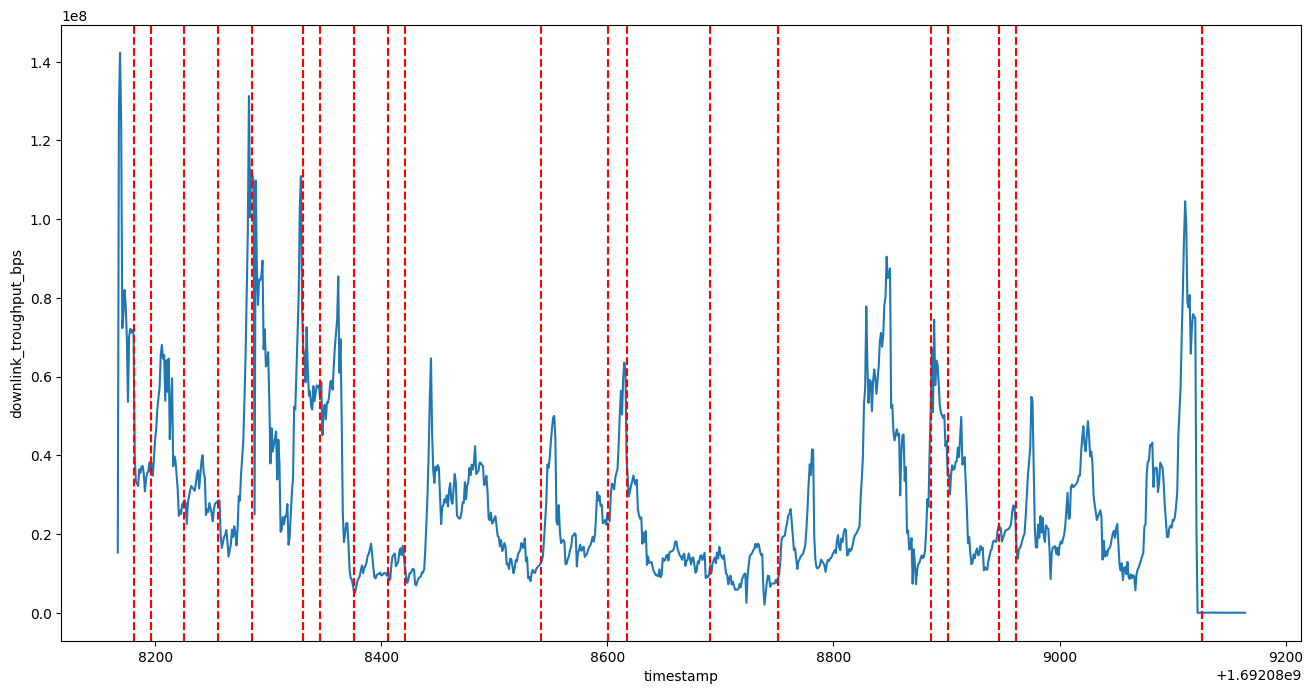
\includegraphics[width=1\columnwidth]{img/correlation_handovers_bw.png}
    \caption{Trying to correlate satellite handovers (red vertical lines) with bandwidth measurements.}
    \label{fig:vis-correlation-handovers}
\end{figure}

As we can verify from Figure \ref{fig:vis-correlation-handovers}, handovers do not seem to impact bandwidth drops. This
suggests the dish is employing a sophisticated technology to perform satellite handovers without leading to a
performance loss, further investigation might be needed to better understand what is enabling smooth transitions between
satellites.

The measurements chapter is, for the moment, concluded; we now move to wrap up our work.


\chapter{Final Remarks and Future Work}

Concluding our experiments, we highlight several key insights. First, the latency to the Point of Presence remains
remarkably stable and low enough even for network-intensive applications, such as online video gaming. In practice, the
average customer, provided they have clear sky access, is usually more than satisfied with Starlink's performances.
Bandwidth is sustained consistently, even in the presence of satellite handovers, which do not appear to impact it
significantly.

Typically, a Starlink dish maintains contact with approximately eight satellites at any given moment, making autonomous
decisions internally about which satellite to connect to. It is worth noting that this satellite count may vary
following new launches.

Unfortunately, obtaining deeper insights into the inner workings of the Autonomous System operated by SpaceX is very
hard. Hosts within this system tend not to respond to standard ping requests, and traceroute data does not always
indicate the path packets take. Another well-protected link in the chain is the dish itself; many of the methods
available are protected and not accessible to the end-user or are deprecated. The dish runs an SSH server, but it is
impossible to connect to it as the manufacturer key pair is needed.

Notably, as of 6 October 2023, Project Kuiper has initiated its satellite launch efforts, thereby advancing its
satellite constellation. By 16 October, the first two Project Kuiper satellites had been fully activated, efficiently
generating power and establishing communication with the mission operations center \cite{kuiplaunches}.

Future research endeavors may include running our measurements over a more extended period. Monitoring changes in
latency and observing potential alterations in traceroutes could provide valuable insights, particularly after the
launch of additional satellites. Given the presence of multiple operators, unusual routing decisions may manifest in the
network's path over time.

Moreover, the methodologies applied in our measurements on Starlink's dish may be adapted for use with Project Kuiper's
dishes as soon as they are commercialized. While specifics about Project Kuiper's dish remain undisclosed, it is
reasonable to expect it to offer a similar API for dish data access.

Additionally, exploring the implementation of an IPv6-compatible router and external access to the dish may facilitate
the execution of diverse measurements, as proposed by Izhikevich et al. \cite{izhikevich2023democratizing}.

Another interesting topic of research are the recently added Inter Satellite Links (ISLs). Detecting whether packets are
relayed between satellites can be accomplished by examining the initial hop after the Starlink Autonomous System. Using
ISL routing might make it cheaper for SpaceX; it is reasonable to assume their operators might want to use their
technology to do some internal routing to later exit the AS, where they have favorable agreements with other service
providers.
    


\appendix
\chapter{Appendix}

\begin{lstlisting}[language=python,label=lst:cvs,caption={the \texttt{calculate\_visible\_satellites} function},captionpos=b]
def calculate_visible_satellites(
    observer_latitude, observer_longitude, observer_elevation, distance_km
):
    stations_url = "https://celestrak.org/NORAD/elements/gp.php?GROUP=starlink&FORMAT=tle"
    satellites = load.tle_file(stations_url)
    observer = Topos(observer_latitude, observer_longitude, observer_elevation)
    ts = load.timescale()
    t = ts.now()

    # Calculate satellite positions
    positions = []
    for sat in satellites:
        satellite = sat
        position = (satellite - observer).at(t)
        positions.append((sat, position))

    # Filter visible satellites
    visible_satellites = []
    for sat, position in positions:
        alt, az, distance = position.altaz()
        # Satellite is above the horizon
        if alt.degrees > 0 and distance.km < distance_km:
            visible_satellites.append((sat, alt, az))

    return visible_satellites
\end{lstlisting}

\chapter{Skyfield Library}
\label{app:sky}

\begin{lstlisting}[language=python,caption={retrieving a Satellite's position using the Satname},captionpos=b]

from skyfield.api import load, wgs84

stations_url = "https://celestrak.org/NORAD/elements/gp.php?GROUP=starlink&FORMAT=tle"
satellites = load.tle_file(stations_url)
print("Loaded", len(satellites), "satellites")
by_name = {sat.name: sat for sat in satellites}
satellite = by_name["STARLINK-1007"]

# year, month, day, hour, minute, second
ts = load.timescale()
t = ts.now()
a = satellite.at(t)
lat, lon = wgs84.latlon_of(a)
print("Latitude:", lat)
print("Longitude:", lon)
\end{lstlisting}

\clearpage
\printbibliography[heading=bibintoc]
\clearpage
\pagestyle{empty}
\end{document}
